% !Mode:: "TeX:UTF-8"

\titlepage

\begin{frame}{说在前面}
	\linespread{1.5}
	  \begin{itemize}[<+-|alert@+>]
	    \item \ba{改错!改错!改错!}
% 	    \item 不记得自己哪周交作业
	  \end{itemize}
\end{frame}

% \begin{frame}{需要注意的问题}
% 	\linespread{1.5}
% 	  \begin{itemize}%[<+-|alert@+>]
% 	    \item L'Hospital法则
% 	    \begin{itemize}
% 	      \item \it 只能应用于“$\df{\bm{0}}{\bm{0}}$”
% 	      和“$\df{\bm{\infty}}{\bm{\infty}}$”型
% 	      \item \it 及时使用无穷小代换进行简化
% 	      \item \it 不正规的符号:\b 
% 	      $\xlongequal{\footnotesize\mbox{“L”}}$、
% 	      $\xlongrightarrow{\footnotesize\mbox{“L'Hospital法则”}}$、
% 	      $\df{\bm{0}}{\bm{0}}$、$\df{\bm{\infty}}{\bm{\infty}}$
% 	    \end{itemize}
% 	    \item Taylor公式
% 	    \begin{itemize}
% 	      \item \it Taylor多项式不包含余项
% 	      \item \it 合并同次幂的系数
% 	      \item \it 尽量按照幂次由低到高排列,最后写余项
% 	    \end{itemize}
% 	  \end{itemize}
% \end{frame}

\section{多元函数的极限与连续}

\begin{frame}
	\linespread{1.5}
	\ba{1.讨论以下二重极限的存在性:
	
	(1)$\lim\limits_{(x,y)\to(0,0)}\df{x+y}{\sqrt{x^2+y^2}}$}
	
	\bigskip
	
	\small 解:\it
	令$x=\rho\cos\theta,y=\rho\sin\theta$,其中$\theta$为常数,则
	$$\lim\limits_{(x,y)\to(0,0)}\df{x+y}{\sqrt{x^2+y^2}}
	=\lim\limits_{\rho\to 0}(\cos\theta+\sin\theta)=\cos\theta+\sin\theta,$$
	注意到右端结果与$\theta$相关,故该二重极限不存在。
	
	\ba{注:在以上解法中将$\theta$视为常数,相当于令$y=kx$,沿折线趋近原点}
\end{frame}

\begin{frame}
	\linespread{1.5}
	\ba{(2)$\lim\limits_{(x,y)\to(0,0)}\df{x+y}{\sqrt{x^2+y^2}}$}
	
	\bigskip
	
	\small 解:\it
	令$x=\rho\cos\theta,y=\rho\sin\theta$,则
	$$\lim\limits_{(x,y)\to(0,0)}\df{xy}{|x|+|y|}
	=\lim\limits_{\rho\to0}\df{\rho\cos\theta\sin\theta}{|\cos\theta|+|\sin\theta|},$$
	注意到$|\cos\theta|+|\sin\theta|\geq\sqrt2$,故对任意$\e>0$,令
	$\delta=\sqrt2\e$,则对任意$0<|\rho|<\delta$,总有
	$$\left|\df{\rho\cos\theta\sin\theta}{|\cos\theta|+|\sin\theta|}\right|
	\leq\df{\rho}{\sqrt2}<\e,$$
	由此可知,该二重极限存在。\fin
	
	\ba{注:证明极限存在时,不可简单地将$\theta$视为常数,否则与沿着$y=kx$趋近原点没有区别。
	仅仅证明沿着$y=kx$趋近时极限相同不能说明二重极限存在!}
\end{frame}

\begin{frame}
	\linespread{1.5}
	\ba{2.计算以下二重极限:}

	\bigskip
	
	\small 解:
	
	(1)$\lim\limits_{(x,y)\to(0,1)}\df{\ln(1+xy)}{y\sin x}
	=\lim\limits_{(x,y)\to(0,1)}\df{xy}{yx}=1.$
	
	(2)$\lim\limits_{(x,y)\to(0,0)}\df{1-\cos(xy)}{(x^2+y^2)e^{x^2}}
	=\lim\limits_{(x,y)\to(0,0)}\df{\frac12x^2y^2}{(x^2+y^2)}$
	
	$\quad\quad=\df12\lim\limits_{x\to
	0}\lim\limits_{y\to0}\df{x^2y^2}{x^2+y^2}=0.$
	
	(3)$\lim\limits_{(x,y)\to(0,0)}\df{e^{xy}-1}{\sqrt{2-e^{xy}}-1}
	=\lim\limits_{(x,y)\to(0,0)}\df{xy}{\frac12(1-e^{xy})}$
	
	$\quad\quad=-2\lim\limits_{(x,y)\to(0,0)}\df{xy}{xy}=-2.$
	\fin
	
	\ba{提示:合理使用无穷小代换可简化多重极限的运算。对于多重极限,不能
	随便使用L'Hospital法则!}
\end{frame}

\section{偏导数与全微分}

\begin{frame}
	\linespread{1.5}
	\ba{1.证明:$f(x,y)=\left\{\begin{array}{ll}
  	(x^2+y^2)\sin\df1{x^2+y^2}, & (x,y)\ne(0,0)\\
  	0, & (x,y)=(0,0)
  \end{array}\right.$
  的偏导函数在原点处不连续,但$f(x,y)$在原点处可微。}
	\pause

% 	\bigskip
	\small 证:\it
	$$f'_x(0,0)=\lim\limits_{\Delta x\to 0}
	\df{(\Delta x)^2\sin\frac1{(\Delta x)^2}-0}{\Delta x}=0,$$
	同理$f'_x(0,0)=0$。
	当$(x,y)\ne(0,0)$时,由偏导数的求导法则,
	$$f'_x(x,y)=2x\sin\df1{x^2+y^2}-\df{2x}{x^2+y^2}\cos\df1{x^2+y^2},$$
	$$f'_y(x,y)=2y\sin\df1{x^2+y^2}-\df{2y}{x^2+y^2}\cos\df1{x^2+y^2}.$$
\end{frame}

\begin{frame}
	\linespread{1.5}
	
	\small \it 偏导函数
	$$f'_x(x,y)=\left\{\begin{array}{ll}
  	2x\sin\df1{x^2+y^2}-\df{2x}{x^2+y^2}\cos\df1{x^2+y^2}, & (x,y)\ne(0,0)\\
  	0, & (x,y)=(0,0)
    \end{array}\right.$$
    注意到累次极限
	$$\lim\limits_{x\to 0}\lim\limits_{y\to 0}
	f'_x(x,y)
	=\lim\limits_{x\to 0}
	\left[2x\sin\df1{x^2}-\df{2}{x}\cos\df1{x^2}\right]
	=-\lim\limits_{x\to 0}
	\df{2}{x}\cos\df1{x^2}$$
	不存在,故二重极限$\lim\limits_{(x,y)\to(0,0)}f'_x(x,y)$
	不存在,从而可知偏导函数$f'_x(x,y)$在原点处不连续。
	
	同理可证$f'_y(x,y)$在原点处不连续。
\end{frame}

\begin{frame}
	\linespread{1.5}
	
	\small \it 进一步,注意到极限
	\begin{align*}
		&\lim\limits_{(x,y)\to(0,0)}\df{f(\Delta x,\Delta y)-f'_x(0,0)\Delta x
		-f'_y(0,0)\Delta y}{\sqrt{(\Delta x)^2+(\Delta y)^2}}\\
		&=\lim\limits_{(x,y)\to(0,0)}\sqrt{(\Delta x)^2+(\Delta y)^2}
		\sin\df1{(\Delta x)^2+(\Delta y)^2}=0,
	\end{align*}
	故
	$$f(\Delta x,\Delta y)-f'_x(0,0)\Delta x-f'_y(0,0)\Delta y
	=\circ(\sqrt{(\Delta x)^2+(\Delta y)^2}),$$
	也即$f(x,y)$在原点处可微。\fin
	
	\ba{要点:讨论二重极限的存在性!可微的证明方法!}
\end{frame}

\begin{frame}
	\linespread{1.5}
	\ba{2.求$z=\arctan\df{x+y}{1-xy}$的所有二阶偏导数。}
	\pause

% 	\bigskip
	\small 解:\it
	注意到
	$$\arctan\df{x+y}{1-xy}=\arctan x+\arctan y,$$
	故
	\begin{align*}
		&z'_x=\df1{1+x^2},\quad\quad\quad
		z'_y=\df1{1+y^2},\\
		&z''_{xx}=-\df{2x}{(1+x^2)^2},\quad
		z''_{yy}=-\df{2y}{(1+y^2)^2},\\
		&z''_{xy}=z''_{yx}=0.
	\end{align*}
	\fin
\end{frame}

\begin{frame}
	\linespread{1.5}
	\ba{3.已知$\df{\p z}{\p y}=\df{x^2+y^2}y$,$z(x,1)=e^x$,
	求$z(x,y)\;(y\ne0)$。}
	\pause

% 	\bigskip
	\small 解:\it
	由$\df{\p z}{\p y}=\df{x^2+y^2}y=\df{x^2}y+y$,可知
	$$z(x,y)=x^2\ln|y|+\df12y^2+u(x),$$
	其中$u(x)$是某个关于$x$的一元函数。又$z(x,1)=e^x$,也即
	$$e^x=\df12+u(x)\quad
	\Rightarrow\quad u(x)=e^x-\df12,$$
	故
	$$z(x,y)=x^2\ln|y|+\df12(y^2-1)+e^x.$$
	\fin
\end{frame}

\begin{frame}
	\linespread{1.5}
	\ba{4.设$z=\dint_x^{xy}e^{(t-x)^2}\d t$,
	求$\df{\p z}{\p x}$和$\df{\p z}{\p y}$。}
	\pause

% 	\bigskip
	\small 解:\it
	令$u=t-x$,则
	$$z=\dint_0^{x(y-1)}e^{u^2}\d u.$$
	进而
	$$
		z'_x=(y-1)e^{x^2(y-1)^2},\quad z'_y=xe^{x^2(y-1)^2}.
	$$
	\fin
	
	\ba{提醒:不要忘记变限积分求导的基本方法!}
\end{frame}

\begin{frame}
	\linespread{1.5}
	\ba{5.求函数$z=xy^2$在$(1,2)$附近且$(\Delta x,\Delta y)=(0.1,-0.5)$时
	对应的函数值的改变量(全增量)与全微分。}
	
% 	\bigskip
	
	\small 解:\it 
	全增量
	$$\Delta z=z(1.1,1.5)-z(1,2)=-1.525,$$
	注意到$z'_x(1,2)=z'_y(1,2)=4$,故全微分
	$$\d z=z'_x(1,2)\Delta x+z'_y(1,2)\Delta y
	=4\cdot 0.1+4\cdot(-0.5)=-1.6.$$
	\fin
	
	\ba{注意:$x,y$为自变量,故$\d x=\Delta x,\d y=\Delta y$,
	给定了$\Delta x,\Delta y$的值,微分的值是可以具体计算出来的!}
\end{frame}

\begin{frame}
	\linespread{1.5}
	\ba{6.利用微分计算$\sqrt{1.02+(1.97)^3}$的近似值。}
	
	\small 解:\it
	考虑函数$z=\sqrt{x+y^3}$,则
	$$z(1,2)=3,\quad z'_x(1,2)=\df16,\quad z'_y(1,2)=2.$$
	进而可知
	$$\sqrt{1.02+(1.97)^3}
	\approx z(1,2)+z'_x(1,2)\cdot0.02+z'_y(1,2)\cdot(-0.03)
	\approx 2.943.$$
	\fin
\end{frame}

\section{补充例题}

\begin{frame}
	\linespread{1.5}
	\ba{例:设$u=u(x)$由
	$$u=f(x,y),\;g(x,y,z)=0,\;h(x,z)=0$$
	确定,$f,g,h$一阶偏导连续,$h'_z\ne0,g'_y\ne0$,求$\df{\p u}{\p x}$}
\end{frame}

\begin{frame}
	\linespread{1.5}
	\ba{例:设$f(u)$当$u>0$时二阶可导,且$z=f(\sqrt{x^2+y^2})$满足方程
	$$\df{\p^2z}{\p x^2}+\df{\p^2z}{\p y^2}=0,$$
	\begin{enumerate}[(1)]
% 	  \setlength{\itemindent}{1cm}
	  \item 证明:$uf''(u)+f'(u)=0$;
	  \item 设$f(1)=0,f'(1)=1$,求$f(u)$。 
	\end{enumerate}}
\end{frame}

\begin{frame}
	\linespread{2}
	\ba{例:设$u(x,y)$满足
	$$\df{\p^2 u}{\p x^2}-\df{\p^2 u}{\p y^2}
	+k\left(\df{\p u}{\p x}+\df{\p u}{\p y}\right)=0.$$
	试选择合适的$a,b$,使得通过变换$u(x,y)=v(x,y)e^{ax+b}$后,所得
	新的方程不再含有任何偏导数项。}
\end{frame}

% \begin{frame}{出现的问题}
% 	\linespread{1.5}
% 	  \begin{itemize}%[<+-|alert@+>]
% 	    \item 作业进度慢!
% 	    \item 概念问题
% 	    \begin{itemize}
% 	      \item \b\it 幂级数展开不熟练
% 	      \item \b\it Maclaurin级数和关于$(x-x_0)$的幂级数分不清
% 	    \end{itemize}
% 	    \item 过程不规范或不完整
% 	    \begin{itemize}
% 	      \item \b\it 求收敛域要单独讨论端点的敛散性
% 	      \item \b\it 相同幂次的项要合并,并按幂次从小到大排列
% 	      \item \b\it 书写潦草随意\pause
% 	    \end{itemize}
% 	    \item \ba{雷同!!!}
% 	  \end{itemize}
% \end{frame}

% \begin{frame}
% 	\linespread{1.5}
% 	\ba{3.设$D$是由曲线$y=\sin x+1$与三条直线$x=0,x=\pi,y=0$
% 	所围成的曲边梯形,求$D$绕$x$轴旋转一周所围成的旋转体的体积。
% 	}
% 	\pause
% 	
% % 	\bigskip
% 	
% 	\begin{columns}
% 		\begin{column}{.5\textwidth}
% 			\begin{center}
% 				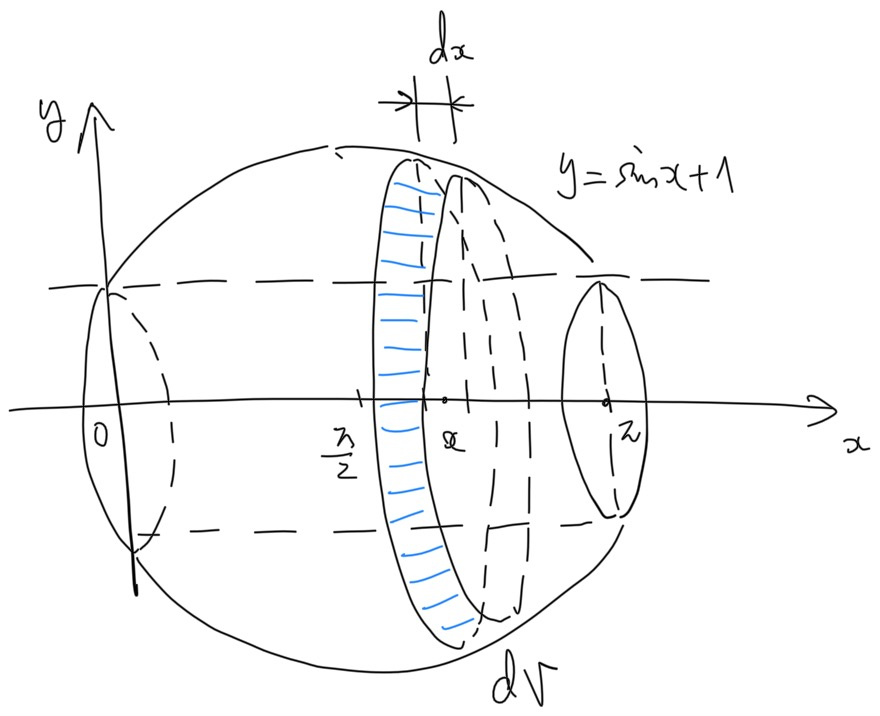
\includegraphics[width=.9\textwidth]{./images/ch6/sinx1cs.jpg}
% 		% 		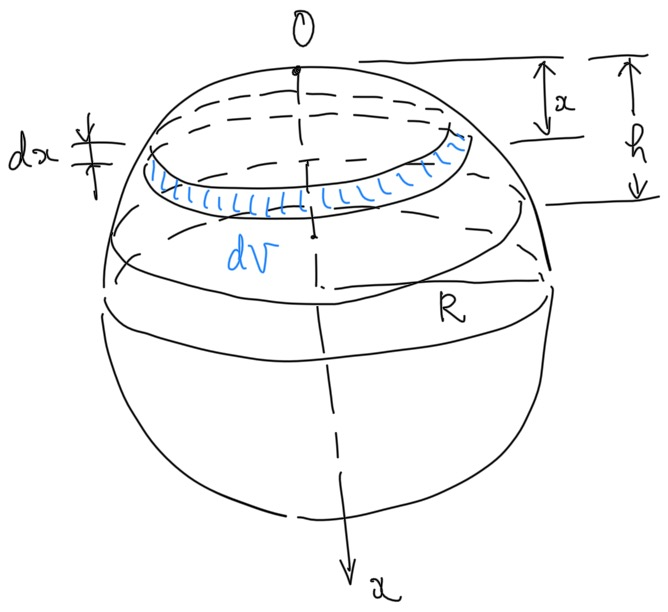
\includegraphics[width=6cm]{./images/ch6/topSp.jpg}
% 			\end{center}		
% 		\end{column}
% 		\begin{column}{.5\textwidth}
% 			\small 解:\it
% 			如图,体积微元$\d V=\pi y^2\d x$,	故所求体积
% 			$$
% 				V=\dint_0^{\pi}\pi(\sin x+1)^2\d x=\df32\pi^2.
% 			$$
% 		\end{column}
% 	\end{columns}
% \end{frame}